\section{Implementacja Systemu WSN/RT}

\newtheorem{rt_book_def}{Definicja "książkowa"}[section]
\newtheorem{rt_practic_def}{Definicja "praktyczna"}[section]
\subsection{Systemy Real Time}
\subsubsection{Podstawowe pojęcia}

\par
\tab Definicja pojęcia bezpieczeństwa systemów czasu rzeczywistego odbiega znacznie od  bezpieczeństwa rozumianego w kontekście klasycznych systemów operacyjnych lub tego z którym spotykamy się podczas problemów związanych z IT-Security. \\
Czym w takim razie jest Real-Time?

\begin{rt_book_def}
Poprawność wykonania operacji
zależy nie tylko od tego, czy
wykonała się bez błędów i zwróciła
poprawny rezultat, ale także od czasu
(górnego ograniczenia) w jakim
operacja się zakończyła.
\end{rt_book_def}

Oznacza to, że o funkcji/operacji możemy powiedzieć że jest czasu rzeczywistego jeśli oprócz tego że wykonany wynik jest "bezbłędny" to również czas wykonania jest z góry określony przez pewne maximum. 

\begin{rt_practic_def}
System RT, to taki, w którym da się
udowodnić, że każda wymagana
operacja zakończy się w określonym
czasie.
\end{rt_practic_def}

W idealnym przypadku jest to dowód matematyczny. Niestety
przy złożoności współczesnych systemów w większości przypadków jest to niewykonalne,
a nawet jeżeli, to istnieje ryzyko popełnienia błędu podczas
dowodzenia. \\
\tab W praktyce stosuje się zestaw testów. System, który przejdzie
takie testy określne w specyfikacji lub powstające podczas jego
tworzenia, jest określany jako system czasu rzeczywistego. 
Testy takie przeprowadza się mierząc czas odpowiedzi na badany sygnał przy otaczających
niekorzystnych dla systemu warunkach, jeśli czas odpowiedzi (deadline) jest deterministyczny to wtedy możemy sądzić że system przeszedł testy pomyślnie.\\

\textbf{Deadline} systemu czasu rzeczywistego nazywamy "Punkt w czasie, w którym dana akcja ma nastąpić (np. reakcja na zmianę stanu wejścia)."

Ze względu na podział systemów czasu rzeczywistego na podgrupy (Hard-RT, Soft-RT) rozróżniamy różnice w pojmowaniu Deadline. \\

\textbf{Hard Real-Time} - operacja zawsze \textbf{musi} zakończyć się w
określonym czasie. Wynik operacji zakończonej później - nie nadaje
się do wykorzystania (awaria już nastąpiła). \\

\textbf{Soft Real-Time} - okazjonalnie operacja \textbf{może} zakończyć się po
ustalonym czasie (błąd nie jest krytyczny dla operacji). \\

Czas pomiędzy momentem w którym akcja miała wystąpić, a momentem w którym w rzeczywistości wystąpiła nazywamy \textbf{opóźnieniem} systemu-RT (Latency). 
W idealnym przypadku (taki system nie istnieje) - opóźnienia
byłyby zerowe. W rzeczywistości komputer potrzebuje pewnego czasu na
ustabilizowanie i przetworzenie sygnałów ze sprzętu,
oprogramowanie wprowadza własne opóźnienia itp. \\ \\
\textbf{Jitter}: wariancja opóźnienia (poprzedniej wartości). Z powodu, że czas pomiędzy wystąpieniem przerwania (zgłoszeniem przez sprzęt) a uruchomieniem procedury jego obsługi nie jest stały mamy doczynienia z wariancją czasów opóźnień, jej zmienność jest równie groźna jak duże opóźnienie (na
przykład uniemożliwia wykorzystanie systemu do akwizycji danych). \\ \\

\textbf{Predictability} Przewidywalność: oznacza wiedzę na temat tego ile czasu zajmie operacja (na
przykład procedura obsługi przerwania).
Teoria algorytmów zajmuje się określaniem złożoności
obliczeniowej poszczególnych metod. W szczególności aby system
był przewidywalny, konieczne jest używanie algorytmów
działających w stałym czasie (niezależnym od ilości danych). \\ 

\textbf{Worst Case} Najgorszy przypadek : ze względu na zmienność rzeczywistych systemów (nie da się zbudować systemu idealnego), głównym polem naszych
zainteresowań pozostaje „najgorszy możliwy przypadek”.
System będzie działał w sposób przewidywalny jeżeli będziemy
znać jego opóźnienie w najgorszym możliwym przypadku.
\clearpage

\subsubsection{Sygnały wejścia/wyjścia}

\par
\tab W ogólnym przypadku systemy cyfrowe lub mikrokontrolerowe oddziaływują ze światem zewnętrznym za pomocą portów wejścia/wyjścia. Porty te mogą być połączone do zewnętrznych czujników i stanowić, magistrale cyfrowe za pomocą których jednostka centralna (mikroprocesor, układ fpga) otrzymuje sygnały pochodzące ze świata zewnętrznego które są zbierane przez czujniki, czy linie za pomocą których mikrokontroler zbiera i analizuje sygnał elektryczny w postaci napięciowej i samodzielnie konwertuje sygnał do postaci cyfrowej. \\
\tab O ile możliwości dostarczania informacji jest bardzo wiele ponieważ istnieje niezliczona ilość czujników które można podłączyć do systemu cyfrowego, istnieją dwa główne sposoby reakcji systemu mikroprocesorowego na zmianę sygnału wejściowego nie zależnie czy odczyt z portu wejścia jest informacją cyfrową czy analogową. Ponieważ każda informacja i tak finalnie jest przetwarzana do postaci cyfrowej rozróżniamy: \textit{wejścia próbkowane ciągle} oraz \textit{wejścia sterowane przerwaniami}.

\par
\tab Wejścia ciągle próbkowane (continuous sampling port detection). W najprostrzej wersji metodę tę można przedstawić z programistycznego punktu widzenia jako nieskończoną pętle w której procesor odczytuje co okreśnoną jednostkę czasu synchronicznie stan komórki pamięci w której jest przechowywany odczyt z zewnętrznego czujnika, i porównuje tę wartość z jakąś inną wartością i w zależności od wyniku porównania następuje określona akcja. \\ 

\centerline{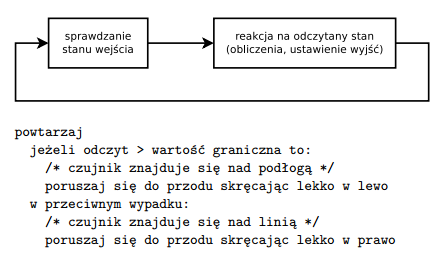
\includegraphics[scale=0.75]{./img/target_system/continius_sampling.png}}
\centerline{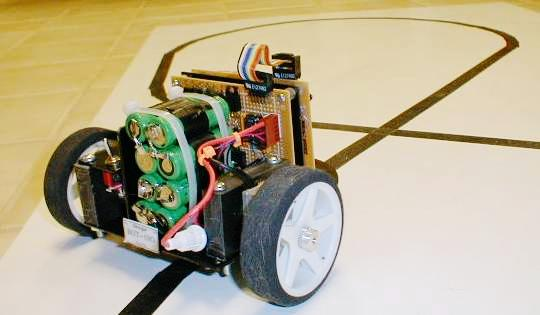
\includegraphics[scale=0.35]{./img/target_system/line_following_robot.jpg}}

\par
\tab Wejścia sterowane przerwaniami są natomiast asynchronicznym sposobem reagowania na zdarzenie przychodzące z zewnątrz. System wykonuje program główny w oderwaniu od zdarzeń zewnętrznych do czasu nadejścia przerwania które wywłaszcza czas procesora na krótki okres podczas którego musi zostać obsłużone. Często takie przerwania są właśnie sygnałami czasu rzeczywistego które przychodzą nagle w odpowiedzi na jakieś zewnętrzne zdarzenie i muszą być jak najszybciej obsłużone. \\ 

\centerline{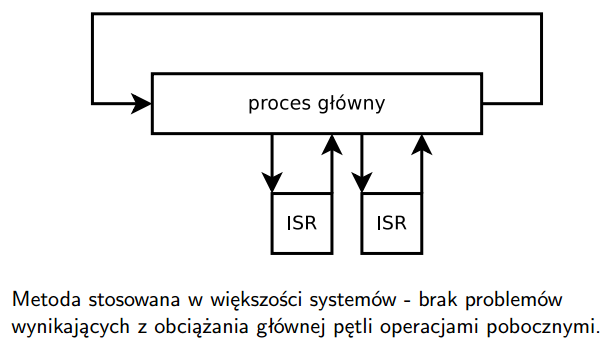
\includegraphics[scale=0.50]{./img/target_system/interrupt_driven_port.png}}

\par 
\tab Najprostrzym układem wzorcowym którym posłużymy się do opisu układu czasu rzeczywistego będzie prosty układ elektryczny zawierający przełącznik dwustanowy (wł/wył) oraz diodę LED. W momencie kiedy zewrzemy przełącznik (stan wł) dioda momentalnie się zapali ponieważ przez zwarty przełącznik zacznie płynąć prąd. 

 \centerline{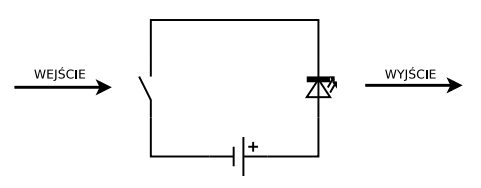
\includegraphics[scale=0.50]{./img/target_system/RT_wzorzec_led.png}}
Układ ten niewątpliwie spełnia wymagania systemów czasu rzeczywistego jednak w praktyce jest trywialny i zbyt ograniczony funkcjonalnie w przemysłowych zastosowaniach. Systemy którymi się zajmujemy posiadają układy mikroprocesorowe, dlatego stwórzmy odpowiednik tego trywialnego układu wykorzystując mikrokontroler.

 \centerline{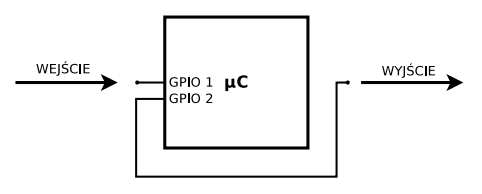
\includegraphics[scale=0.50]{./img/target_system/uc_RT_gpio.png}}
 
 Rozważany układ może pełnić rolę pokazanego wyżej prostego połączenia przełącznika do zewnętrznego odbiornika np diody led. Wejście mikrokontrolera jest wzbudzane sygnałem i system reaguje zmieniając stan wyjścia. W tym przypadku są to PIN-y GPIO ale sytuacja niczym się nie różni od wzbudzania wejścia przy pomocy innego (wewnętrznego mechanizmu). Np odczytywaniu stanu czujnika cyfrowego lub wartości napięcia, co w przypadku mechanicznego przełącznika byłoby niemożliwe. Systemy mikroprocesorowe dają nam dużo więcej możliwości niż układy oparte o mechaniczne rozwiązania, oraz co najważniejsze wypadają dużo lepiej w przypadku szybkich sygnałów niż jakiekolwiek mechaniczne zamienniki. Wymagają one jednak innego podejścia podczas testowania niż ich mechaniczne odpowiedniki ponieważ przebieg programu może być różny w zależności od warunków zewnętrznych. \\
 \centerline{\includegraphics[scale=0.10]{./img/target_system/rt_signal.png}}


\subsubsection{Definicja systemu RT na potrzeby pracy}

\par 
\tab Systemem czasu rzeczywistego w dalszej części pracy będziemy nazywali taki system operacyjny który spełnia wymagania określone jako "Hard real time" czyli dla każdej zdefiniowanej funkcjonalności posiada ograniczony z góry czasowy deadline.
Funkcjonalności są to w przypadku ogólnym wszystkie możliwe funkcje systemu których argumentami są zewnętrzne parametry. Funkcja taka musi dawać jakiś wynik, ponieważ musi być mierzalna. Funkcjonalności systemu mogą być wykorzystywane bezpośrednio przez użytkownika którym może być człowiek, inny system lub badane zjawisko.

\par
\tab Dodatkowo na potrzeby niniejszej pracy zakładamy, że każda z funkcjonalności jest przewidywalna czyli z góry znamy średni czas wykonania operacji. Przykładowo wiemy, że po naciśnięciu guzika w przeciągu pół sekundy zapali się dioda.
Kolenją cechą badanych dalej systemów czasu rzeczywistego jest wartość Jitter-a (wariacji opóźnienia) chcemy badać takie systemy w których Jitter nie jest funkcją losową a stanowi sumę różnych czynników zewnętrznych mających wpływ na wykonywanie operacji/funkcjonalności, z zastrzeżeniem że wartości tych czynników mogą mieć losową wartość w czasie (np wpływ promieniowania elektromagnetycznego w postaci fal radiowych na układ) jednak wartość ta jest ograniczona przez pewne normy (np normy dotyczące dopuszczalnego promieniowania elektromagnetycznego w mieście) lub ograniczenia przyrody (maksymalna/minimalna temperatura, wilgotność powietrza).

\par
\tab Powyższe założenia mają na celu wyodrębnienie takich systemów w których największe i znaczenie mają kwestię techniczne i inżynieryjne, natomiast nie skupia się na analizie opartej o zbyt głębokie matematyczne kwestię takie jak zaawansowana statystyka czy rachunek prawdopodobieństwa.

\clearpage